\documentclass[11pt,a4paper,english,hyperref]{article}
\usepackage[utf8]{inputenc}

\newcommand\blattNummer{12}
\newcommand\abgabeDatum{24.5.2019}
\newcommand\ersteAufgabeNummer{1}

%%%%%%%%%%%%%%%%%%%%%%%%%%%%%%%%%%%%%%%%%%%%%%%%%%%%%%%%%%%%%%%%%%%%%%%%%% 
\usepackage{babel}
\usepackage{exscale}
\usepackage{amsmath,amsfonts,amssymb}
\usepackage[thref, amsmath, amsthm, thmmarks]{ntheorem}
\usepackage{a4wide}
\usepackage{epic,eepic}
\usepackage{graphicx} % einbinden von Grafiken mit \includegraphics
\usepackage{url}
\usepackage{mathtools}
\usepackage{etoolbox}
\usepackage[colorlinks]{hyperref}
\usepackage{enumitem}
\usepackage[capitalize]{cleveref}
\usepackage{enumitem}

\pagestyle{empty}
\parindent0em
\parskip1ex
\addtolength{\topmargin}{0cm}
\addtolength{\oddsidemargin}{0cm}
\addtolength{\textheight}{2cm}
\addtolength{\textwidth}{0cm}

% neuer Zähler für die Aufgaben
\newcounter{aufgabeNummer}
\setcounter{aufgabeNummer}{\ersteAufgabeNummer}
\addtocounter{aufgabeNummer}{-1}

% in enumerate-Umgebungen erst Kleinbuchstaben, dann kleine römische Zahlen
\renewcommand{\labelenumi}{(\alph{enumi})\,}
\renewcommand{\labelenumii}{(\roman{enumii})\,}
\setenumerate[0]{label=(\alph*)}
\crefname{enumerate}{}{}

% Stil für Definitionen, Sätze usw.
\theoremstyle{break}   % Titelzeile abgesetzt
\newtheorem{Satz}{Proposition}
\newtheorem{Lemma}{Lemma}
\newtheorem{Definition}{Definition}
\theorembodyfont{\upshape}  % normaler Font f"ur Beispiel, Aufgabe
\newtheorem{Beisiep}{Example}
\newtheorem{Aufgabe}[aufgabeNummer]{Exercise}

\theoremstyle{definition}
\newtheorem{remark}{Remark}

% Mathematische Kürzel
\newcommand\R{\mathbb{R}}
\newcommand\Q{\mathbb{Q}}
\newcommand\N{\mathbb{N}}
\newcommand\Z{\mathbb{Z}}
\renewcommand\P{\mathbb{P}}
\newcommand\T{{\mathcal T} }

\newcommand\eps{{\varepsilon}}                                  % machine precision?
\newcommand\im{{\sl i\;}}                                        % imaginary unit?
\newcommand\e{{\rm e}}                                          % Euler number
\newcommand\D{{\rm D\;}}
\DeclarePairedDelimiter\abs{\lvert}{\rvert}
\DeclarePairedDelimiter\norm{\lVert}{\rVert}
\DeclarePairedDelimiter\dotProductD{\langle}{\rangle}           % Delimiters for dot product

\DeclareMathOperator{\spann}{span}
\DeclareMathOperator{\cond}{cond}
\DeclareMathOperator{\round}{round}
\DeclareMathOperator{\supp}{supp}

\begin{document}
\parbox{0ex}{ \scalebox{.27}{  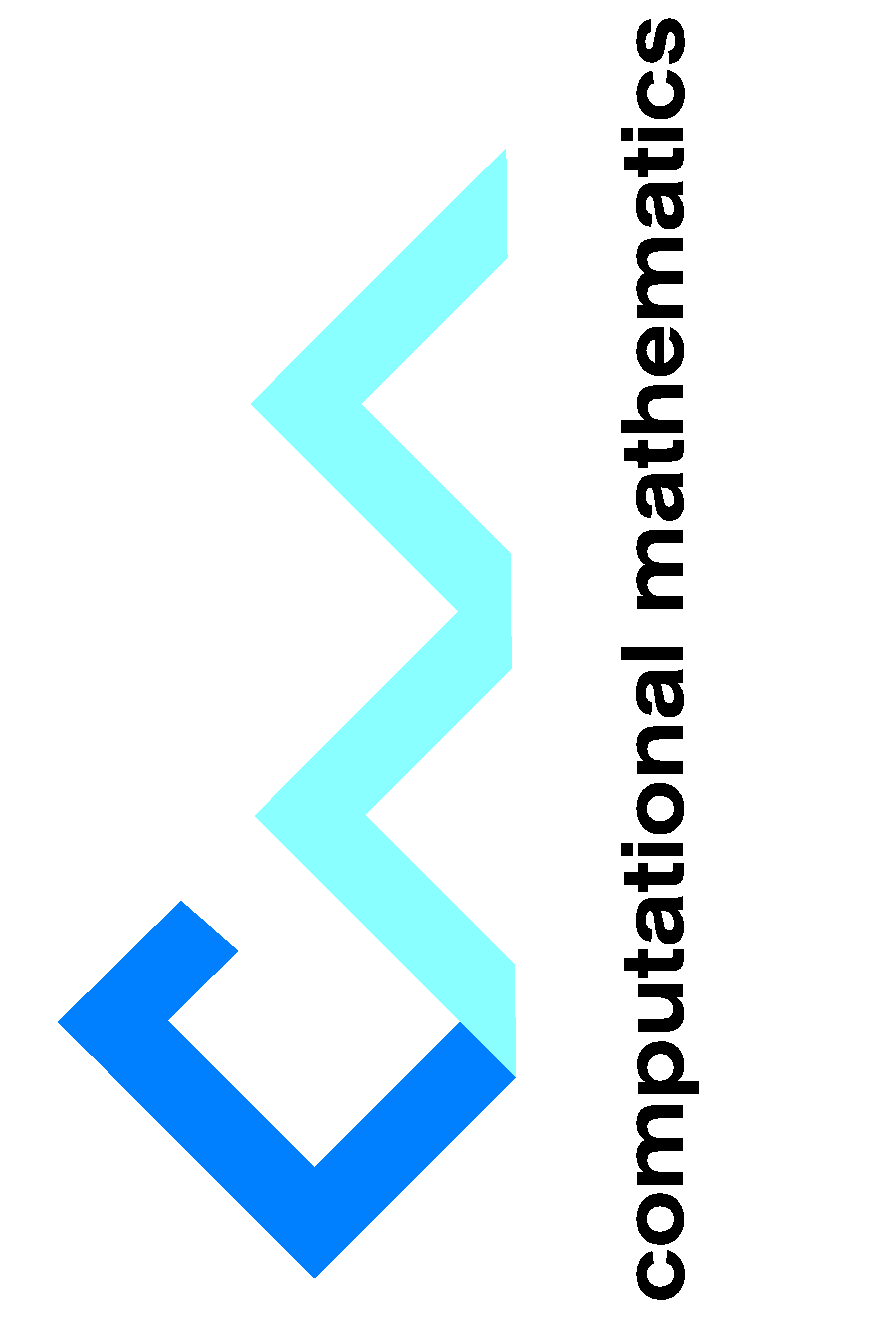
\includegraphics[width=.5\textwidth,angle=-90]{cm-logo2.eps} }   }   \\
\parbox{25ex}{
  Prof.~Dr.~S.~Sauter\\
  Institut für Mathematik\\
  Universität Zürich
}
% 
\rule[0cm]{0.cm}{.01cm}                  
\hfill  \parbox{0.6\textwidth}{
  {\sf\LARGE\bfseries Numerik I}
  {\sf\Large\bfseries \;\;--\;\; Homework \blattNummer }\\[1.5ex]
  Deadline: \abgabeDatum,\ 13:00
}
\vspace{5ex}

\begin{Aufgabe}[2 Points, Theoretical task]
  Prove Proposition 8.17 from the lecture notes: the Richardson method
  \begin{equation*}
    x^{(m+1)}\coloneqq  \left( I-\omega A \right) x^{(m)} + \omega b
  \end{equation*}
  converges with maximal order (i.e. $\frac{\norm{x^{(m+1)} -x^{*}}}{\norm{x^{(m)} -x^{*}}}$ is minimal, where $x^*$ is the exact solution) if $\omega=\frac{2}{\lambda_{\max}+\lambda_{\min}}$.
\end{Aufgabe}
\begin{Aufgabe}[9 Points, Computational task]
  \begin{enumerate}
    \item (3 points) Implement the Richardson and SOR iterative solver for the linear system $Ax=b$:
    your functions should take as input the matrix $A$ and vector $b$, the parameter $\omega$, a starting vector and optionally the desired tolerance.
    \item (1 point) Use your code from the previous exercise sheet, or the functions provided on the course page, to compute the matrix $M$ and vector $r$ for $10$ grid points on each dimension;
    use the explicit eigenvalues expression given in the script to compute the parameter $\omega_{opt}$ for the Richardson method.
    \item (3 points) Use the functions you just implemented to solve the system $Mu=r$ with the Richardson and Gauss-Seidel (i.e. SOR with $\omega=1$) methods. Choose the zero vector as starting vector.
    Compare the convergence rate of the two methods, i.e. the ratio $e_{i+1}/e_i$, where $i$ is the iteration index and $e_i$ is the residuum: $e_i \coloneqq M u^{(i)} - r$.
    \item (2 points) Keeping the starting vector fixed, test your SOR method for different values of $\omega$, and experimentally determine $\omega_{opt}$ for which the number of iterations required to obtain convergence is the smallest.
  \end{enumerate}
\end{Aufgabe}
\begin{remark*}
  Iterative methods are particularly useful when using sparse matrices. However, we don't ask you to use data structures for sparse matrices in your implementation, and we measure the complexity by the number of matrix-vector multiplications.
\end{remark*}
\begin{Aufgabe}[4 points, Theoretical task]
  A function $u\in C^{1}\left( \mathbb{R} \right)$ is identically zero for all $x \leq 0$. Given a step size $h > 0$, we define the grid points $x_{i}=ih$, $i\in\mathbb{Z}$.
  \begin{enumerate}
    \item Using polynomial interpolation, construct a formula for the approximation of $u^{\prime}\left( x_{i}\right)$ by determining the coefficients $\alpha_{0}$, $\alpha_{1}$, $\alpha_{2}$ in
    \begin{equation*}
      \alpha_{0} u\left(x_{i}\right)  +\alpha_{1}u\left(  x_{i-1}\right) + \alpha_{2}u\left(  x_{i-2}\right)
    \end{equation*}
    \item Derive an error estimate for this approximation, assuming that the function is smooth.
  \end{enumerate}
\end{Aufgabe}
\end{document}